\PassOptionsToPackage{unicode=true}{hyperref} % options for packages loaded elsewhere
\PassOptionsToPackage{hyphens}{url}
%
\documentclass[ignorenonframetext,aspectratio=54,]{beamer}
\usepackage{pgfpages}
\setbeamertemplate{caption}[numbered]
\setbeamertemplate{caption label separator}{: }
\setbeamercolor{caption name}{fg=normal text.fg}
\beamertemplatenavigationsymbolsempty
% Prevent slide breaks in the middle of a paragraph:
\widowpenalties 1 10000
\raggedbottom
\setbeamertemplate{part page}{
\centering
\begin{beamercolorbox}[sep=16pt,center]{part title}
  \usebeamerfont{part title}\insertpart\par
\end{beamercolorbox}
}
\setbeamertemplate{section page}{
\centering
\begin{beamercolorbox}[sep=12pt,center]{part title}
  \usebeamerfont{section title}\insertsection\par
\end{beamercolorbox}
}
\setbeamertemplate{subsection page}{
\centering
\begin{beamercolorbox}[sep=8pt,center]{part title}
  \usebeamerfont{subsection title}\insertsubsection\par
\end{beamercolorbox}
}
\AtBeginPart{
  \frame{\partpage}
}
\AtBeginSection{
  \ifbibliography
  \else
    \frame{\sectionpage}
  \fi
}
\AtBeginSubsection{
  \frame{\subsectionpage}
}
\usepackage{lmodern}
\usepackage{amssymb,amsmath}
\usepackage{ifxetex,ifluatex}
\usepackage{fixltx2e} % provides \textsubscript
\ifnum 0\ifxetex 1\fi\ifluatex 1\fi=0 % if pdftex
  \usepackage[T1]{fontenc}
  \usepackage[utf8]{inputenc}
  \usepackage{textcomp} % provides euro and other symbols
\else % if luatex or xelatex
  \usepackage{unicode-math}
  \defaultfontfeatures{Ligatures=TeX,Scale=MatchLowercase}
\fi
% use upquote if available, for straight quotes in verbatim environments
\IfFileExists{upquote.sty}{\usepackage{upquote}}{}
% use microtype if available
\IfFileExists{microtype.sty}{%
\usepackage[]{microtype}
\UseMicrotypeSet[protrusion]{basicmath} % disable protrusion for tt fonts
}{}
\IfFileExists{parskip.sty}{%
\usepackage{parskip}
}{% else
\setlength{\parindent}{0pt}
\setlength{\parskip}{6pt plus 2pt minus 1pt}
}
\usepackage{hyperref}
\hypersetup{
            pdftitle={Edward Glaeser: A városgazdaságtan diadala},
            pdfauthor={Koren Miklós},
            pdfborder={0 0 0},
            breaklinks=true}
\urlstyle{same}  % don't use monospace font for urls
\newif\ifbibliography
\usepackage{graphicx,grffile}
\makeatletter
\def\maxwidth{\ifdim\Gin@nat@width>\linewidth\linewidth\else\Gin@nat@width\fi}
\def\maxheight{\ifdim\Gin@nat@height>\textheight\textheight\else\Gin@nat@height\fi}
\makeatother
% Scale images if necessary, so that they will not overflow the page
% margins by default, and it is still possible to overwrite the defaults
% using explicit options in \includegraphics[width, height, ...]{}
\setkeys{Gin}{width=\maxwidth,height=\maxheight,keepaspectratio}
\setlength{\emergencystretch}{3em}  % prevent overfull lines
\providecommand{\tightlist}{%
  \setlength{\itemsep}{0pt}\setlength{\parskip}{0pt}}
\setcounter{secnumdepth}{0}

% set default figure placement to htbp
\makeatletter
\def\fps@figure{htbp}
\makeatother

\usepackage{pgfpages}
\usepackage{microtype}
\usepackage{tikz}
  \usetikzlibrary{positioning}
  \usetikzlibrary{arrows}
  \usetikzlibrary{graphs}

\definecolor{CTred}{RGB}{229,32,32}
\definecolor{CTgrey}{RGB}{153,153,153}

\usepackage{array}
\usepackage{dcolumn}
\newcolumntype{d}{D{.}{.}{-1}}
\usepackage{booktabs}
\usepackage{threeparttable}

% colors: white text on 90% black background
\setbeamercolor{normal text}{fg=black,bg=white}

% light blue as a highlight color
\setbeamercolor*{structure}{fg=CTred}
\setbeamercolor{section title}{fg=CTred}
\setbeamercolor{alerted text}{use=structure,fg=CTred}
\setbeamercolor*{palette primary}{use=structure,fg=structure.fg}
\setbeamercolor*{palette secondary}{use=structure,fg=structure.fg!95!black}
\setbeamercolor*{palette tertiary}{use=structure,fg=structure.fg!90!black}
\setbeamercolor*{palette quaternary}{use=structure,fg=structure.fg!95!black,bg=black!80}

\setbeamercolor*{framesubtitle}{fg=white}


% use system fonts: here, Gill Sans
\usefonttheme{professionalfonts}
\setbeamerfont{quote}{shape=\upshape}

% eliminate silly beamer navigation line at bottom of slides
\setbeamertemplate{navigation symbols}{}
\setbeamertemplate{footline}[frame number]

% ensure text jusfication
\usepackage{ragged2e}
\justifying

% pandoc makes 2nd-lever headers into blocks, and this ensures justification
% in blocks too
\addtobeamertemplate{block begin}{}{\justifying}




\urlstyle{same}
\usepackage[overlay,absolute]{textpos}

\setbeamertemplate{items}[square]

\TPGrid[10 mm,8 mm]{9}{8}
% beamer's left and right margin is 10 mm. The top/bottom margin is ??
% or without a header ??
% the slide dimensions are 128 mm x 96 mm
% so the resulting \TPHorizModule = 12 mm and \TPVertModule = 10 mm

% uncomment if you want biblatex for citations on slides

% \usepackage{csquotes}
% \usepackage[notes,short,noibid,backend=biber]{biblatex-chicago}
% \bibliography{course.bib} 

\providecommand{\exhibit}[2]{\includegraphics[keepaspectratio, height=0.9\textheight, width=\textwidth]{assets/img/#1}\\ {\tiny #2}}

\providecommand{\smallcite}[1]{({\footnotesize #1})}

\title{Edward Glaeser: A városgazdaságtan diadala}
\author{Koren Miklós}
\date{2023. november 16.}

\begin{document}
\frame{\titlepage}

\begin{frame}{Mennyi az ideális népsűrűség?}
\protect\hypertarget{mennyi-az-ideuxe1lis-nuxe9psux171rux171suxe9g}{}

\pause

\begin{block}{Várostervező}

\ldots{}, \ldots{} (oszt, szoroz) \ldots{} 1,100 fő/km\({}^2\)

\pause

\end{block}

\begin{block}{Közgazdász}

Attól függ! Mennyi a lakbér? Milyen az infrastruktúra? Milyen
munkalehetőségek vannak?

\end{block}

\end{frame}

\begin{frame}{1. Bevezetés}
\protect\hypertarget{bevezetuxe9s}{}

\begin{itemize}
\tightlist
\item
  \textbf{Fókusz}: Edward Glaesert a városok érdeklik. Városok
  növekedése és hanyatlása, az agglomeráció okai és következményei,
  szakpolitikai beavatkozások, történelmi példák.
\item
  \textbf{Háttér}: PhD Chicago 1992. Harvard University 1992--. 162 ezer
  hivatkozás.
\end{itemize}

\end{frame}

\begin{frame}{2. Egyedülálló Fókusz a Városi Dinamikára}
\protect\hypertarget{egyeduxfcluxe1lluxf3-fuxf3kusz-a-vuxe1rosi-dinamikuxe1ra}{}

\begin{itemize}
\tightlist
\item
  \textbf{Városok Fejlődése és Hanyatlása}: Emberi tőke és oktatás
  fontossága. A városok növekedése szorosan kapcsolódik a tudás és az
  innováció központi szerepéhez. A városok hanyatlását gyakran a
  gazdasági diverzifikáció hiánya, a merev szabályozások és a társadalmi
  problémák okozzák.
\item
  \textbf{Agglomeráció Gazdaságtana}: Emberi interakciók és az
  információcsere hatékonysága. Jobb munkalehetőségekhez való
  hozzáférés, a szolgáltatások és infrastruktúra koncentrációja, de
  magasabb megélhetési költségek és a forgalmi dugók.
\end{itemize}

\end{frame}

\begin{frame}{Michaels, Rauch és Redding 2019}
\protect\hypertarget{michaels-rauch-uxe9s-redding-2019}{}

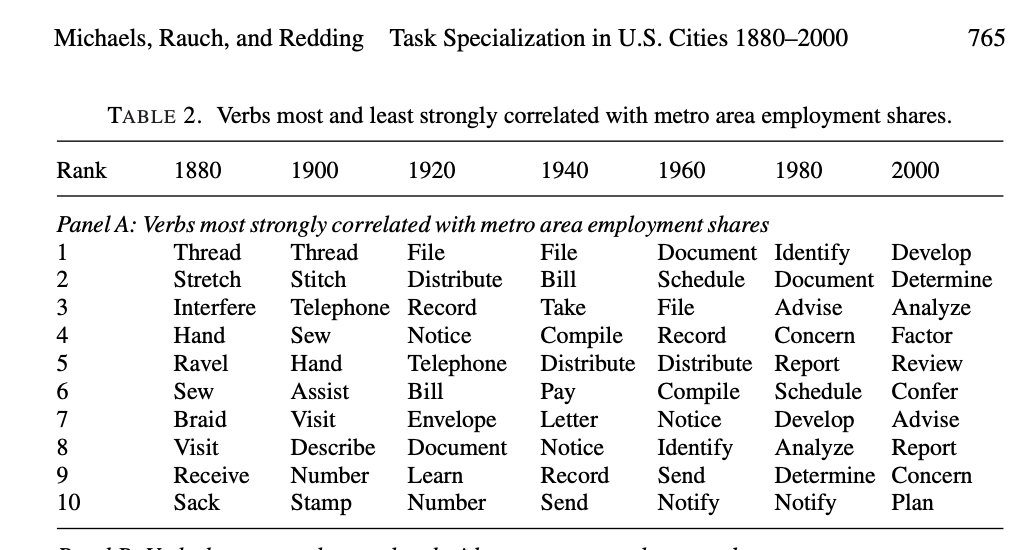
\includegraphics{michaels2019.png}

\end{frame}

\begin{frame}{3. Változatos Módszertan}
\protect\hypertarget{vuxe1ltozatos-muxf3dszertan}{}

\begin{itemize}
\tightlist
\item
  \textbf{Mikroadatok Elemzése}: Háztartási és vállalati census,
  ingatlanadatok, földrajzi adatok, GIS.
\item
  \textbf{Multidiszciplináris Megközelítés}: Közgazdaságtan, ökonometria
  (pl. jobb null modellek), földrajz, történelem, város-szoicológia.
\end{itemize}

\end{frame}

\begin{frame}{Ellison és Glaeser 1997 (JPE)}
\protect\hypertarget{ellison-uxe9s-glaeser-1997-jpe}{}

Geographic Concentration in U.S. Manufacturing Industries: A Dartboard
Approach

A tradicionális koncentráció-mérőszámok fölfele torzítanak. Kevés
telephely \(\to\) látszólagos koncentráció még akkor is, ha
véletlenszerű a telephelyek térbeli eloszlása (dartboard approach).

\end{frame}

\begin{frame}{4. Tudás Bizonytalanság Idején}
\protect\hypertarget{tuduxe1s-bizonytalansuxe1g-idejuxe9n}{}

Sokan nem mernek bizonytalanság idején előrejelezni. (Nincs rá adat!
Nincs rá kísérlet!)

De mikor jelezzünk előre, ha nem akkor, amikor senki nem tud semmit?

\begin{itemize}
\tightlist
\item
  \textbf{9/11}: Modellek és történelmi példák alapján: a nagyvárosok
  ellenállnak még az ilyen nagy sokkoknak is.
\item
  \textbf{Covid-19}: Valószínűbb hosszútávú hatás. (Cutler és Glaeser
  2021, Survival of the City.)
\end{itemize}

\end{frame}

\begin{frame}{5. Következtetés}
\protect\hypertarget{kuxf6vetkeztetuxe9s}{}

Glaeser fókuszált, de nem szakbarbár. Még akkor sem, ha Chicagóban
végzett. (\emph{There are no libertarians in cities.})

És nem fél előrejelzéseket tenni.

\end{frame}

\end{document}
